\title{Поддержка встроенных языков \\ в интегрированных средах разработки}
%
\titlerunning{Поддержка встроенных языков}

\author{Иванов Андрей Васильевич}
%
\authorrunning{А.В.Иванов} % abbreviated author list (for running head)
%
%%%% list of authors for the TOC (use if author list has to be modified)
\tocauthor{А.В.Иванов}
%
\institute{Санкт-Петербургский государственный университет\\
\email{ivanovandrew2004@gmail.com}}

\maketitle              % typeset the title of the contribution
\section*{Введение}

Программы, написанные на современных языках программирования, во время выполнения могут формировать 
выражения на других языках и выполнять их. Языки, которые используются для написания таких динамически 
формируемых выражений, называются встроенными. 

Несмотря на то что сегодня широко распространено использование таких технологий, как ORM (object-relational mapping), 
есть области, в которых встроенные языки встречаются достаточно часто. В качестве примера можно привести реинжиниринг 
программного обеспечения. 

Ниже приведен пример использования встроенных языков.

\begin{figure}[h]
\label{PHP}
\centering
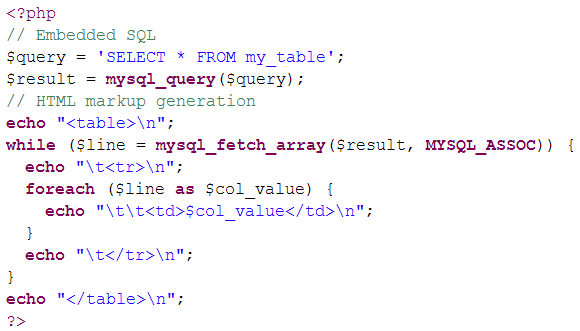
\includegraphics[width=\linewidth]{Ivanov/Pictures/PHP.png}
\caption{Использование нескольких различных встроенных в PHP языков (MySQL, HTML)}
\end{figure}

При работе с приложениями, содержащими встроенные языки, необходимо помнить, что порождаемые строки тоже могут являться кодом на некотором языке программирования. Поэтому важно сохранить синтаксическую корректность динамически формируемых выражений. 

Одна из основных трудностей в работе со встроенными языками заключается в том, что часто отсутствуют средства разработки, позволяющие определить правильность составленного динамического выражения статическим образом, то есть до запуска основной программы. Это связано с тем, что компилятором такие выражения воспринимаются как простые строки.

С другой стороны, сегодня при создании ПО активно используются интегрированные среды разработки --- IDE (Integrated Development Environment), которые предоставляют набор различной функциональности, позволяющей значительно упростить процесс создания программ. Примером могут служить такие функции, как автодополнение, рефакторинг (улучшение написанного ранее кода, не влияющее на его внешнее поведение), дополнительные статические проверки, подсказки. 

Такие возможности современных IDE были бы полезны и для встроенных языков, поскольку это позволило бы сократить время на создание, отладку и сопровождение приложений, использующих динамически формируемые выражения.  К примеру, подсветка синтаксиса могла бы сигнализировать о правильно набранной синтаксической конструкции или же о допущенной опечатке. 

В данной работе представлено механизм поддержки произвольных встроенных языков, описанных грамматикой, для среды разработки Microsoft Visual Studio\footnote{http://www.visualstudio.com}, а также описание реализации этого механизма. 

\section{Обзор}
\subsection{Обзор существующих инструментов}
На данный момент существует ряд инструментов, которые могут работать со встроенными языками. 

Они кратко описаны ниже. 
\begin{itemize}
\item
{
    PhpStorm\footnote{http://www.jetbrains.com/phpstorm}~--- интегрированная среда разработки для PHP, которая осуществляет подсветку и автодополнение встроенного кода на HTML, CSS, JavaScript, SQL. Но эта поддержка осуществляется не для всех строчек. На рисунке~\ref{PHPStorm} правые части присваиваний переменных \$hello1 и \$hello2 ``распознаны'' и подсвечены как выражения на языке HTML. Однако про переменную \$hello3 такого сказать нельзя.

\begin{figure}[t]
\centering
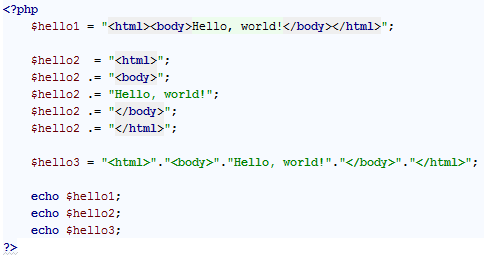
\includegraphics[width=\linewidth]{Ivanov/Pictures/PHPStorm.PNG}
\caption{Пример поддержки встроенных языков в PHPStorm.}
\label{PHPStorm}
\end{figure}
}
\item
{
    IntelliLang\footnote{http://www.jetbrains.com/idea/webhelp/intellilang.html}~--- плагин к средам разработки PHPStorm и IntelliJ IDEA\footnote{http://www.jetbrains.com/idea}, c помощью которого для каждого строкового выражения можно указать, на каком языке оно написано. Например, IntelliLang для PHPStorm поддерживает различные диалекты языков запросов к базам данных. К недостаткам плагина следует отнести то, что для каждого строкового выражения нужно указывать язык явным образом.
}
\item
{
В статье Hyunha Kim, Kyung-Goo Doh and David Schmidt~\cite{Kim} описан инструмент, осуществляющий статическую валидацию HTML-страниц, которые порождаются программами на PHP и JSP. К достоинствам инструмента является то, что валидация осуществляется как синтаксическая, так и семантическая. К примеру, этот инструмент может указывать на такие ошибки, как отсутствие обязательного атрибута, наличие двух разных элементов с одинаковым id и другие.
}
\item
{
    Alvor\footnote{https://code.google.com/p/alvor}~--- это плагин к среде разработки Eclipse, который проверяет корректность встроенных SQL-выражений в код на Java. Ищет динамические выражения на SQL и проверяет их на соответствие SQL-грамматике. В случае, когда SQL-запросы содержат синтаксические и семантические ошибки, Alvor подчёркивает соответствующие места в исходном коде и выводит информацию об ошибках до запуска программы. 
}
\item 
{
    Java String Analyzer~\cite{JSA}~--- это инструмент для анализа формирования строковых выражений на Java. Для каждого такого выражения он строит конечный автомат, представляющий приближённое значение всех значений этого выражения, которые могут быть получены во время исполнения. 
}
\item
{
PHP String Analyzer~\cite{PSA}~--- это инструмент для статического анализа строк, порождаемых PHP. Он аппроксимирует значения таких строк контекстно-свободной грамматикой. Это может быть использовано, например, для валидации генерируемых программами на PHP Web-страниц. 
}
\end{itemize}

Все приведённые выше инструменты, за исключением PHPStorm, предназначены для валидации динамически формируемых выражений, но не решают задачи подсветки синтаксиса встроенных языков. PHPStorm и IntelliLang (как вместе, так и по отдельности) решают эту задачу, но не для всех языков. Хотелось бы получить инструмент, который может осуществлять подсветку синтаксиса произвольного встроенного языка, описанного грамматикой.

\subsection{Обзор используемых инструментов}

\subsubsection{YaccConstructor}
На кафедре системного программирования математико-механического факультета СПбГУ разрабатывается инструмент YaccConstructor~\cite{YC_paper}~\footnote{http://code.google.com/p/recursive-ascent}, позволяющий создавать генераторы синтаксических анализаторов под .NET. Основным языком разработки является мультипарадигмальный язык F\#~\cite{FSharp}. Этот инструмент имеет модульную структуру, которая позволяет создавать анализаторы с различными алгоритмами разбора. Один из таких модулей создан для работы со встроенными языками. В рамках этого модуля уже реализованы алгоритмы абстрактного лексического и синтаксического анализа. ``Абстрактный анализ''~\cite{ARNGLR} здесь означает, что в качестве входа анализатор принимает не линейный поток токенов, а некую структуру. 

\begin{figure}[t]
\centering
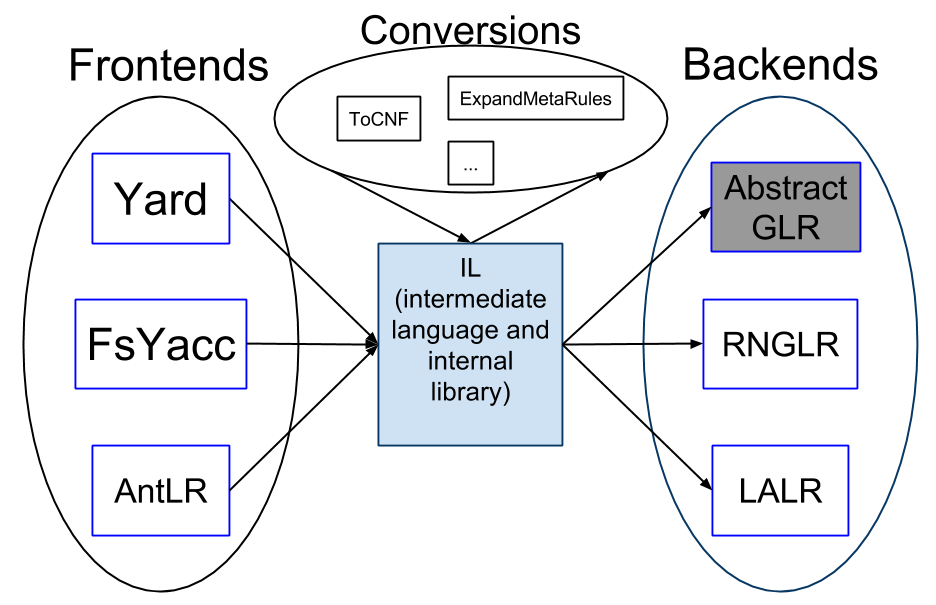
\includegraphics[width=\linewidth]{Ivanov/Pictures/YC_base.png}
\caption{Архитектура YaccConstructor}
\end{figure}

Рассмотрим работу абстрактного синтаксического анализатора чуть подробнее. 
\begin{itemize}
\item
{
На вход анализатору подаётся граф токенов (а не линейная последовательность, как в классическом анализе). Все токены образуют алгебраический тип данных Token, который создаётся генератором. Помимо этого каждый токен содержит в себе некоторую информацию: координаты в исходном файле (что необходимо при подсветке синтаксиса или же при уведомлении об ошибках).
}
\item
{По входному графу токенов строится SPPF~\cite{RNGLR} (Shared Packed Parsed Forest) --- структура, которая позволяет хранить все деревья разбора в сжатом виде. 
}
\item При необходимости можно осуществлять трансляцию деревьев. 
\end{itemize}

\subsubsection{ReSharper SDK}

Компания JetBrains разработала ReSharper --- плагин к Microsoft Visual Studio, который позволяет повысить продуктивность работы, осуществляя дополнительные статические проверки и предоставляя дополнительные средства автодополнения, навигации, поиска и т.п.
У этого плагина есть свой SDK (Software Development Kit).  

Архитектура состоит из нескольких модулей. Рассмотрим некоторые из них.
\begin{itemize}
\item Platform --- модуль, осуществляющий интеграцию с MS Visual Studio. Содержит в себе подмодули для работы с файлами solution, с файлами проектов, с файлами с исходным кодом. 

\item PSI (Project Structure Interface) --- модуль, занимающийся структурой программы: лексический и синтаксический анализ языков, которые поддерживается ReSharper’ом. Содержит в себе компоненту, позволяющую добавлять поддержку новых языков. В данной работе используется PSI модуль используется для получения структуры программы на основном языке.

\item Daemon. Сборки Daemon являются работающими в фоновом режиме потоками, которые анализируют исходный код и реагируют на различные изменения в нём. 
	
\end{itemize}

При запуске программы ReSharper запускает свыше трёхсот сборок, которые осуществляют разнообразный анализ. Для того чтобы одна из этих сборок занималась каким-то самостоятельно реализованным анализом, нужно добавить какой-нибудь атрибут к определению класса (например, [DaemonStage] или [ContextAction]) и унаследоваться от какого-нибудь ReSharper’овского интерфейса (например, IDaemonStage). И тогда при запуске программы ReSharper инстанцирует требуемый класс и будет вызывать его методы при соответствующих изменениях. 

Тип этих изменений может определяться атрибутом. Например, класс, отмеченный атрибутом [DaemonStage], будет заново инстанцироваться при каждом изменении в файле с исходным кодом (например, напечатан или удалён какой-то символ). А если класс отмечен атрибутом [ContainsContextConsumer], то такая реакция будет происходить на каждое изменение положения курсора. 

\section{Алгоритм}
\subsection{SPPF}

SPPF~\cite{RNGLR}~--- структура, позволяющая хранить все деревья разбора в сжатом виде. Идея в том, что деревья разбора имеют много одинаковых вершин. Хранить каждую из них отдельно для каждого дерева~--- не самая лучшая идея, поскольку это плохо скажется на памяти. SPPF позволяет куда экономнее её использовать, так как хранит в себе только один фрагмента какого-то дерева, который в свою очередь может разделяться между несколькими деревьями. 

В классическом синтаксическом анализе эта структура склеивает узлы, соответствующие одинаковым нетерминалам или терминалам, в один  узел, если они принимают одинаковую входную цепочку. Если существует множество различных выводов для одного нетерминала, то множество семейств всех детей разделяет одну родительскую вершину. 

Рассмотрим грамматику: 

\begin{verbatim}
    [<Start>]
    s : a 
    a : p r | u v
    p : B
    u : B
    r : C
    v : C
\end{verbatim}

Эта грамматика неоднозначна, поскольку при входной цепочке ``B C'' будет получено два дерева разбора. 

На рисунке~\ref{sppf_idea} продемонстрировано, как могут быть сжаты полученные деревья.

\begin{figure}[t]
\centering
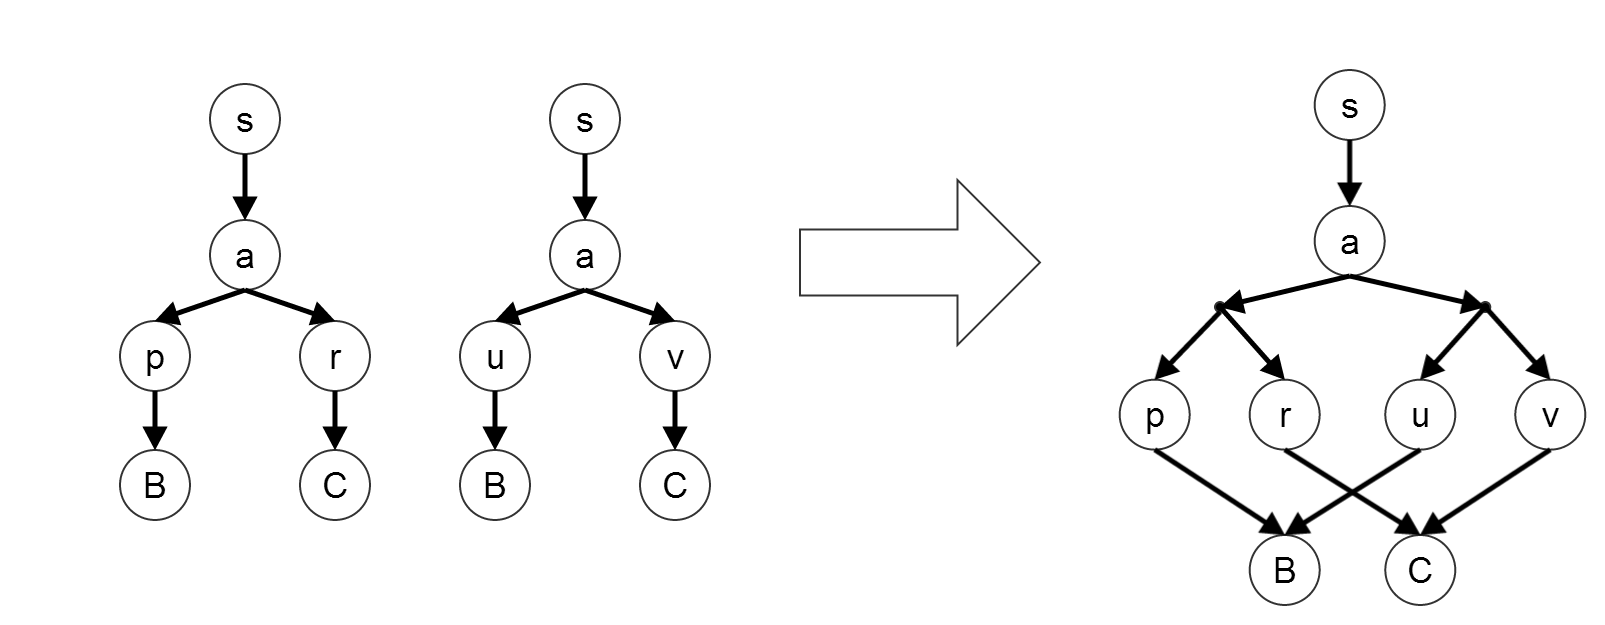
\includegraphics[width=\linewidth]{Ivanov/Pictures/sppf.png}
\caption{Пример получения SPPF из нескольких деревьев.}
\label{sppf_idea}
\end{figure}

Однако в абстрактном синтаксическом анализе возможна ещё одна ситуация. Предположим, что в грамматике только один стартовый нетерминал (если их несколько, то можно добавим новое стартовое правило). Если деревья соответствуют разным путям во входном графе, то из их корневых вершин выводятся разные цепочки. Однако некоторая часть дерева, соответствующая одному или нескольким путям от корня дерева, повторяются у всех деревьев. Поэтому такие вершины тоже предлагается сливать в одну, несмотря на то что формально они могут выводить разные цепочки. 

Поясним на примере такой грамматики.

\begin{verbatim}
    [<Start>] 
    s : a 
    a : b | d 
    b : A B
    d : A D 
\end{verbatim}

Предположим, что на входе у нас граф, изображённый на рисунке~\ref{sppf_input}.

\begin{figure}[t]
\centering
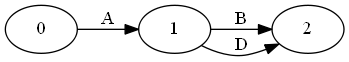
\includegraphics[width=0.5\linewidth]{Ivanov/Pictures/SPPF_input.png}
\caption{Пример входного графа.}
\label{sppf_input}
\end{figure}

Построятся два дерева, у которых пути от вершины s до вершины a будут совпадать (см. рис.~\ref{sppf2}). Несмотря на то что в одном дереве эти вершины выводят строку ``A B'', а в другом ``A D'', вершины этого пути будут также склеены в одну. 

\begin{figure}[t]
\centering
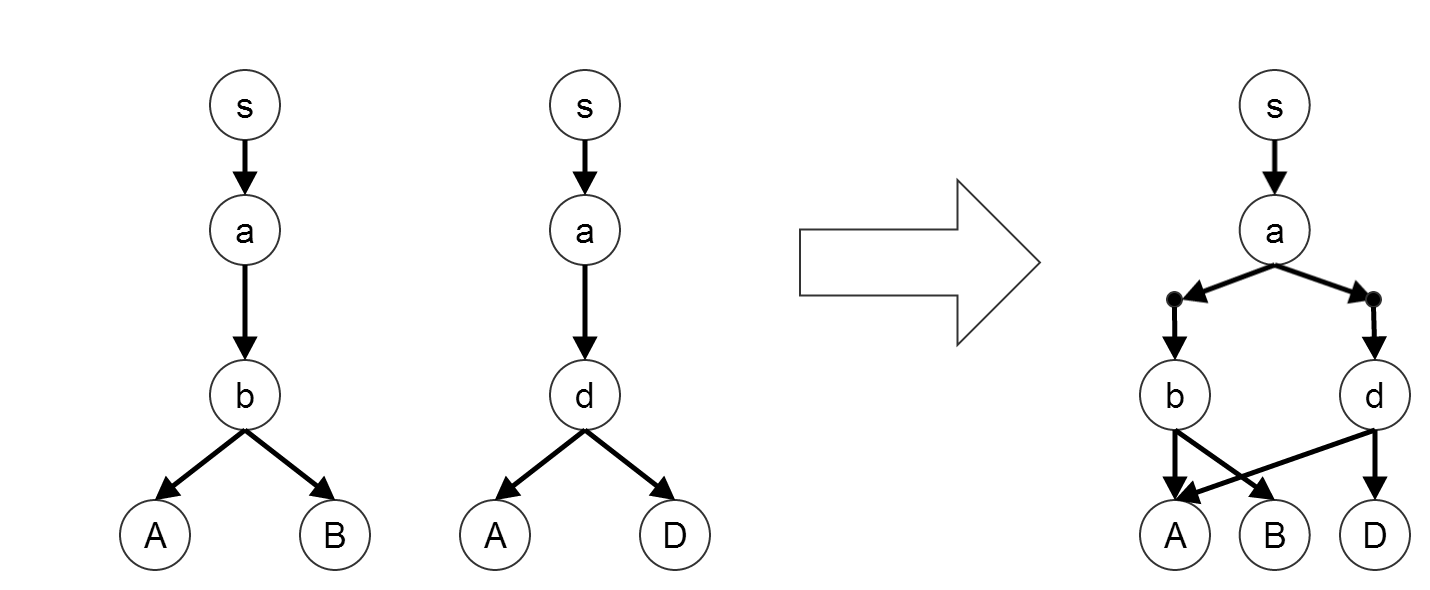
\includegraphics[width=\linewidth]{Ivanov/Pictures/sppf2.png}
\caption{Пример слияния деревьев в SPPF в абстрактном случае.}
\label{sppf2}
\end{figure}

На рисунке~\ref{sppf_yc} показано, как будет выглядеть SPPF для предыдущего примера в реализации YaccConstructor. Заметим, что в реализации YaccConstructor у SPPF помимо привычных узлов, соответствующих терминалам и нетерминалам (далее будем называть их ``вершинами-символами''), есть ещё промежуточные узлы, которые содержат в себе номера продукции (далее будем называть такие вершины ``вершинами-продукциями''). 

\begin{figure}[t]
    \centering
    \subfloat[Первое дерево]{
        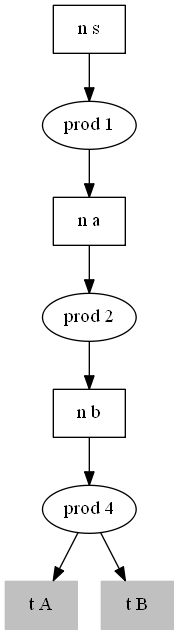
\includegraphics[width=\linewidth]{Ivanov/Pictures/SPPF_YC_ex1.png}
    }
    \qquad
    \subfloat[Второе дерево]{
        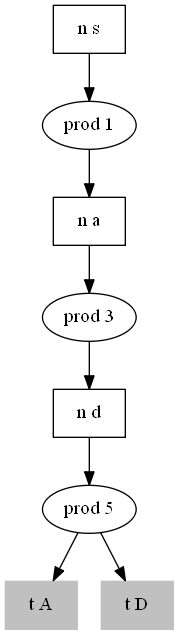
\includegraphics[width=\linewidth]{Ivanov/Pictures/SPPF_YC_ex2.png}
    }
    \qquad
    \subfloat[Результат слияния]{
        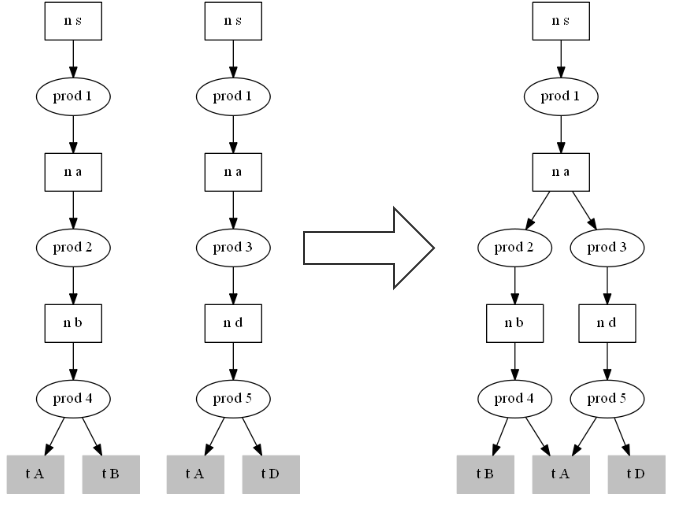
\includegraphics[width=\linewidth]{Ivanov/Pictures/SPPF_YC.png}
    }
    \qquad
    \caption{Слияние деревьев в SPPF в YaccConstructor.}
    \label{sppf_yc}
\end{figure}

Выпишем некоторые свойства SPPF, реализованного в YaccConstructor. 
\begin{itemize}
\item Корни всех деревьев соответствуют одному и тому же нетерминалу. Поэтому при склеивании деревьев будет одна вершина, в которую не входит ни одна дуга. Далее будем называть такую вершину корнем SPPF, или просто корнем. 
\item Все токены располагались на листьях деревьев. В SPPF токены располагаются, т.е. на вершинах, из которых не выходит ни одной дуги.
\item При обходе графа от корня обнаружить вершину-символ, которую разделяют несколько поддеревьев, достаточно просто: из таких вершин выходит более одной дуги к вершинам-продукциям. 
\end{itemize}

Невозможна ситуация, когда SPPF содержит ``лишние деревья'', то есть деревья, для которых нет пути во входном графе. Это свойство вытекает из построения SPPF. 

Пусть $m$ различных поддеревьев склеиваются к вершине, соответствующей одинаковому нетерминалу $n$. Тогда по построению SPPF будет создано $m$ вершин-продукций, к каждой из которых будет вести дуги из $n$. Если в дальнейшем пути от этих вершин-продукций не пересекаются, то никаких новых деревьев появиться не может. 

Таким образом, ``лишнее дерево'' может случиться только в случае, если какие-то деревья имеют общее поддерево. Рассмотрим это поддерево поподробнее. Если оно не содержит в себе неоднозначностей (т.е. ситуации, когда из вершины-символа выходит более, чем одна дуга, к вершинам-продукциям), то мы получим ровно столько же деревьев, сколько и разделяет это поддерево. Поэтому ``лишнего'' дерева в таком случае получиться не может. 

Предположим, что это поддерево содержит в себе неоднозначности и при этом была порождено лишнее дерево. Рассмотрим входной граф (рис.~\ref{sppf_proof_input}). 

Грамматика выглядит так:

\begin{verbatim}
   [<Start>]
   s: a | b
   a: A c
   b: A D c
   c: B | E F
\end{verbatim}

\begin{figure}[t]
\centering
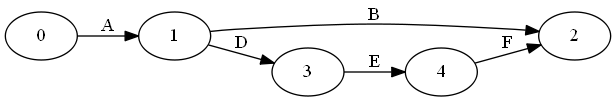
\includegraphics[width=\linewidth]{Ivanov/Pictures/SPPF_proof_input.png}
\caption{Входной граф.}
\label{sppf_proof_input}
\end{figure}

\begin{figure}[t]
    \centering
    \subfloat[Первое дерево]{
        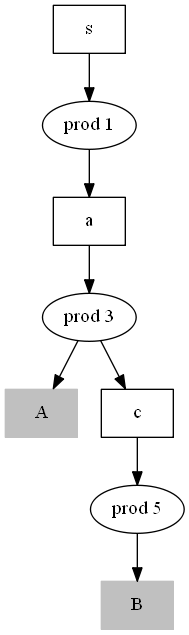
\includegraphics{Ivanov/Pictures/SPPF_proof_fst}
    }
    \qquad
    \subfloat[Второе дерево]{
        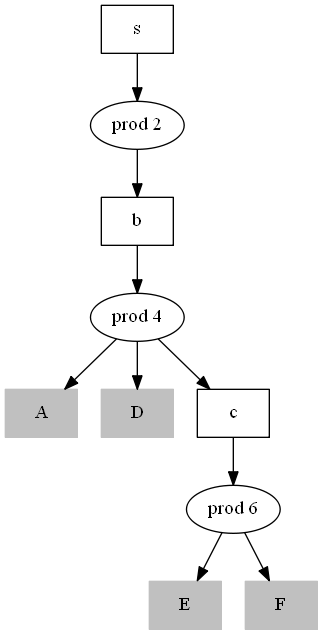
\includegraphics{Ivanov/Pictures/SPPF_proof_snd}
    }
    \qquad
    \subfloat[Слияние деревьев]{
        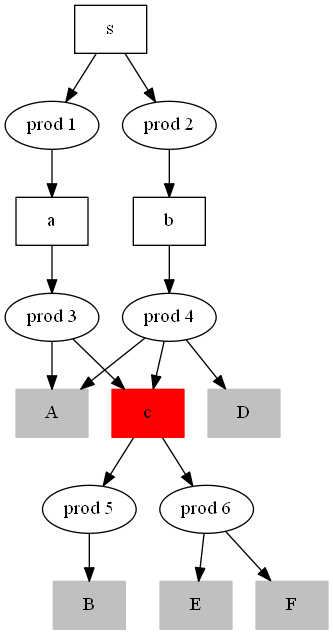
\includegraphics{Ivanov/Pictures/SPPF_proof_incorrect.png}
    }
\caption{Неправильное слияние деревьев.}
\label{sppf_proof_incorrect}
\end{figure}

В возможном SPPF (рисунок~\ref{sppf_proof_incorrect}) два дерева (одно порождает строку ``A B'', а другое --- строку ``A D E F'') имеют общее поддерево, начинающееся с вершины c. Причём это поддерево содержит в себе два разных поддерева: одно порождает строку ``B'', а другое --- строку ``E F''. Таким образом, мы можем получить сразу четыре дерева разбора, которые выводят такие строки:
\begin{itemize}
\item ``A B'',
\item ``A E F'',
\item ``A D B'',
\item ``A D E F''.
\end{itemize}

Причём только для первого и четвёртого случая существуют пути в графе. 

Но граф разбора, изображённый на рисунке~\ref{sppf_proof_incorrect}, получиться не может. Потому что нарушается требование того, что вершины сливаются в одну, если они выводят одинаковую цепочку. В данном случае это требование нарушено: в одном дереве нетерминал c выводит строку ``B'', а в другом --- строку ``E F''. Поэтому сливать вершины, соответствующие вершинам c, в одну, нельзя. Правильный вариант SPPF изображён на рисунке~\ref{sppf_proof_correct}.

\begin{figure}[t]
\centering
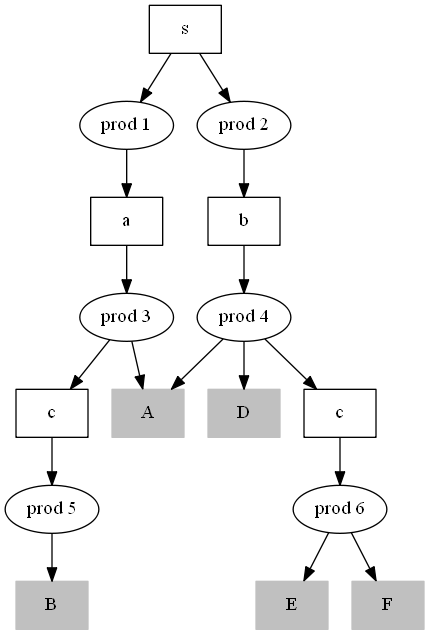
\includegraphics{Ivanov/Pictures/SPPF_proof_correct.png}
\caption{Правильное слияние деревьев.}
\label{sppf_proof_correct}
\end{figure}

Поэтому ситуация, когда общее поддерево, содержащее неоднозначности, приводит к появлению ``лишнего дерева'', невозможна. 

А значит и общая ситуация, когда SPPF содержит в себе дерево, для которого нет пути во входном графе, невозможна.

\subsection{Генерация деревьев из SPPF}
\subsubsection{Статическая подсветка}
При подсветке синтаксиса встроенного языка не обязательно рассматривать все деревья. Достаточно выбрать из леса разбора, полученного синтаксического анализа, подмножество корректных деревьев таким образом, чтобы множество всех токенов (листьев) было покрыто. То есть чтобы для каждого токена существовало дерево из выбранного подмножества, которое содержит этот токен. Действительно, если у двух разных деревьев листья (токены) совпадают, то при подсветке синтаксиса не так уж и важно, какому именно дереву принадлежит тот или иной лист. Важно, что это дерево синтаксически корректно, поскольку над таким деревом можно производить другие действия (например, автодополнение, навигация по коду).

В качестве примера рассмотрим приведённую ниже грамматику и входной граф, изображённый на рисунке~\ref{shift_reduce_conflict}:

\begin{verbatim}
   [<Start>]
   expr: expr PLUS expr 
   expr: NUM
\end{verbatim}

\begin{figure}[t]
\centering
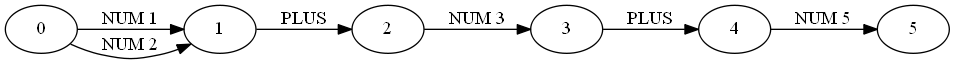
\includegraphics[width=\linewidth]{Ivanov/Pictures/Conflict.png}
\caption{Входной граф, содержащий Shift/Reduce конфликт.}
\label{shift_reduce_conflict}
\end{figure}

Для данного графа в результате синтаксического разбора будет построено целых четыре дерева разбора, т.к. для каждого пути будет построено по два дерева (ввиду неоднозначности грамматики). Однако порождённые конфликтом Shift/Reduce деревья соответствуют одному и тому же пути в графе, а значит, множества их листьев совпадают. Поэтому в данном примере при поддержке подсветки синтаксиса для каждого пути в графе достаточно рассмотреть только одно из таких деревьев. То же самое верно и для Reduce/Reduce конфликта. 

Наиболее сложной для реализации поддержки языков является, соответствующая ветвлению во входном графе. Сложность заключается в том, что в худшем случае для покрытия всех токенов придётся рассматривать все возможные деревья разбора. На рисунке~\ref{bad_case} продемонстрирован пример такого входного графа. 

\begin{figure}[t]
\centering
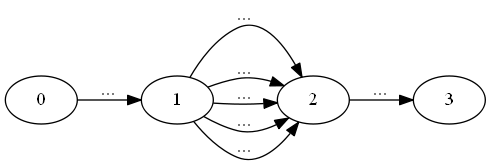
\includegraphics[width=\linewidth]{Ivanov/Pictures/Bad_case.png}
\caption{Входной граф, в котором необходимо рассмотреть все деревья разбора.}
\label{bad_case}
\end{figure}

Однако поскольку в вопросе подсветки деревьев скорость является одним из самых критичных, то принято решение осуществлять генерацию деревьев ленивым образом. Это позволит сэкономить время и память. 

Для того чтобы описать алгоритм извлечения деревьев из SPPF, введём следующие обозначения.
\begin{itemize}
\item OutEdges ($v$)~--- количество исходящих дуг из вершины $v$. 
\item Succ ($v$)~--- $\{u \mid \mbox{существует дуга из вершины } v \mbox{ в вершину u} \}$.
\item Tokens ($v$)~--- количество токенов, которые принадлежат графу с корнем $v$.
\end{itemize}

На вход алгоритму подаётся граф разбора и множество $unprocessed$ --- множество токенов, которые нужно посетить. $root$ = корень графа разбора. Все вершины окрашены в белый цвет. 

Вернуть GetTree (root, unprocessed).

GetTree (v, unprocessed):
\begin{itemize}
\item Если unprocessed = $\emptyset$, то вернуть пустое дерево (null).
\item Иначе вернуть Handle (v, unprocessed).
\end{itemize}

Handle (v, unprocessed):
\begin{enumerate}
\item Если вершина v --- вершина-символ, то 
    \begin{itemize}
        \item Если OutEdges (v) == 0, то это значит, вершина $v$ соответствует какому-то токену $t$. unprocessed = unprocessed $\setminus \{t\}$; 
        \item Если OutEdges (v) == 1, то Handle (Succ (v), unprocessed).
        \item Если OutEdges (v) > 1, то 	$s = arg \; max_{u \in Succ(v)} \; \mid \mbox{Tokens (u)} \cap \mbox{unprocessed} \mid$. Handle (s, unprocessed). // т.е. идём по тому поддереву, которое содержит в себе наибольшее количество токенов из множества unprocessed. 
    \end{itemize}
    Перейти к шагу 3.
\item Если текущая вершина --- вершина-продукция, то для каждой вершины $u \in$~Succ(v) сделать следующее:  Handle (u, unprocessed). Перейти к шагу 3.
\item Покрасить v в чёрный цвет. Если v == root, то перейти к шагу 4.
\item Алгоритм завершает работу. Вернуть дерево, состоящее из ``чёрных'' вершин, и множество unprocessed. 
\end{enumerate}

Рассмотрим работу алгоритма на примере входного графа, изображённого на рисунке~\ref{illustration_input}.

\begin{figure}[t]
\centering
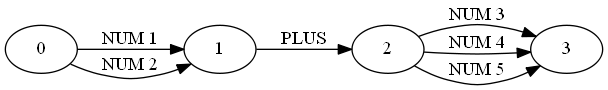
\includegraphics[width=\linewidth]{Ivanov/Pictures/Illustration.png}
\caption{Пример входного графа.}
\label{illustration_input}
\end{figure}

Граф разбора для такого входа будет выглядеть следующим так, как показано на рисунке~\ref{illustration_sppf}.

\begin{figure}[t]
\centering
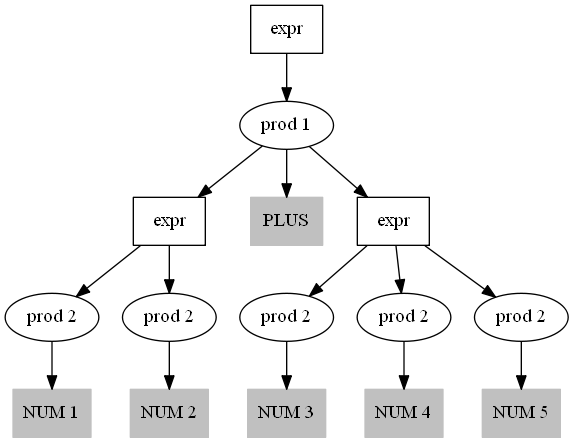
\includegraphics[height=\linewidth]{Ivanov/Pictures/Illustration_sppf.png}
\caption{SPPF для предыдущего примера.}
\label{illustration_sppf}
\end{figure}

При генерации первого дерева из этой структуры у нас все токены считаются непокрытыми. Поэтому алгоритм на вход принимает множество, состоящее из всех токенов. Поскольку любое из шести возможных деревьев разбора содержит три токена, то алгоритм вернёт любое из них. Предположим, что он вернул дерево, изображённое на рисунке~\ref{Illustration_res1}. 

\begin{figure}[t]
    \centering
    \subfloat[Результат первого запуска алгоритма]{
        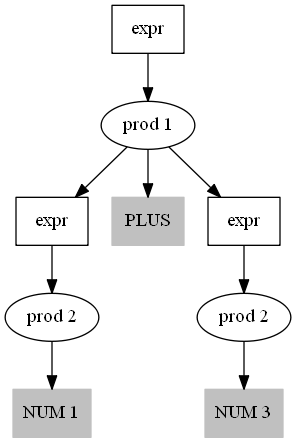
\includegraphics{Ivanov/Pictures/Illustration_res1.png}    
        \label{Illustration_res1}
    }
    \qquad
    \subfloat[Результат второго запуска алгоритма]{
        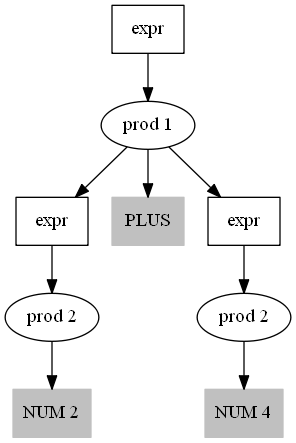
\includegraphics{Ivanov/Pictures/Illustration_res2.png}
        \label{Illustration_res2}
    }
    \qquad
    \subfloat[Результат третьего запуска алгоритма]{
        \centering
        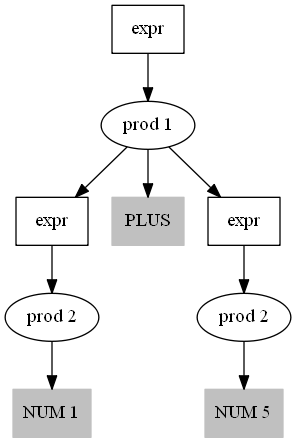
\includegraphics{Ivanov/Pictures/Illustration_res3.png}
        \label{Illustration_res3}
    }
    \caption{Деревья для графа на рисунке~\ref{illustration_sppf}, которые покрывают все токены}
\end{figure}

Также вместе с этим деревом вернётся множество, состоящее из токенов NUM 2, NUM 4 и NUM 5. Это множество передаётся алгоритму при втором запуске. 

На основе этой информации алгоритм снова начинает обход графа с ``корня''. На этот раз существует два дерева, которые содержат в себе два ``новых'' токена (т.е. токена из переданного на вход множества), три дерева, которые содержат в себе один ``новый'' токен, и одно дерево, которое не содержит в себе ``новых'' токенов (то, которое было возвращено при предыдущем запуске). Алгоритм выбирает одно из деревьев, которое содержит в себе наибольшее количество новых токенов (см. рисунок~\ref{Illustration_res2}). Также возвращается множество, состоящее из NUM 5 --- токен, который ещё не покрыли. 

При третьем запуске алгоритм на вход получает множество, состоящее из NUM 5, и снова начинает обход с корня. На этот раз существует четыре дерева, которые не содержат в себе новых токенов, и два дерева, которые содержат в себе один новый токен. И вернёт алгоритм вместе с одним из таких деревьев (например, как на рисунке~\ref{Illustration_res3}) ещё и пустое множество. 

Если запустить алгоритм, передав ему на вход пустое множество, то он вернёт null, не начиная обхода. Это будет означать, что все возможные ``листья'' уже покрыты. 
\subsubsection{Динамическая подсветка}
Современные IDE однако могут осуществлять статическим образом, но и на основе некоторой контекстной информации. Например, если каретка курсора располагается непосредственно перед открывающей скобкой, то эта скобка и парная ей закрывающая скобка могут быть особо выделены цветом. В данной работе такая возможность также реализована. 

В такой задаче уже не все предположение, сделанные в случае статической подсветки, применимы. Добавим в грамматику арифметических выражений правило 

\begin{verbatim}
   expr : LBRACE expr RBRACE
\end{verbatim}

и рассмотрим вход, изображённый на рисунке~\ref{dynamic_idea}. 

\begin{figure}[t]
\centering
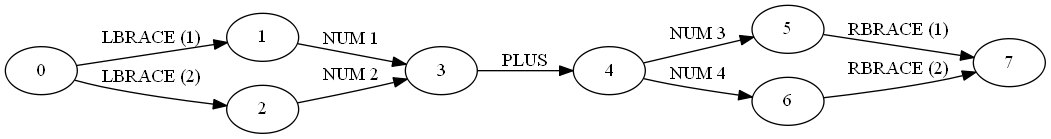
\includegraphics[width=\linewidth]{Ivanov/Pictures/Dynamic_Idea.png}
\caption{Пример получения SPPF из нескольких деревьев.}
\label{dynamic_idea}
\end{figure}

Алгоритм, предложенный в предыдущем разделе, вернёт деревья, изображённые на рисунке~\ref{staticRes}.

\begin{figure}[t]
    \centering
    \subfloat[]{
         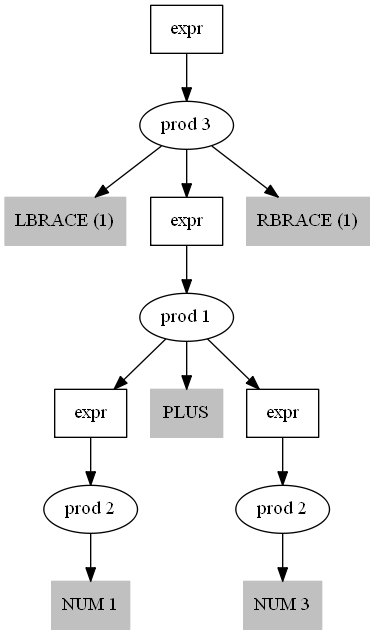
\includegraphics{Ivanov/Pictures/Dynamic_StaticRes1.png}
    }
    \qquad \qquad
    \subfloat{}{
         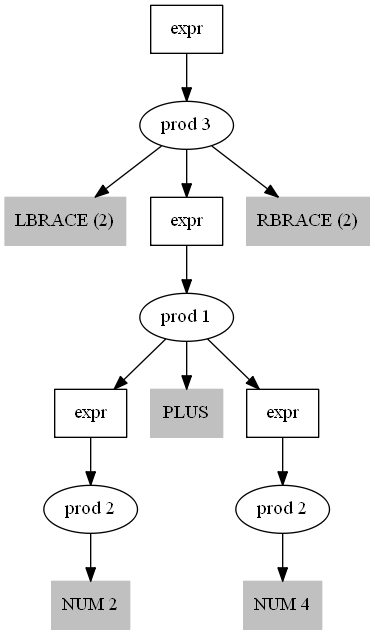
\includegraphics{Ivanov/Pictures/Dynamic_StaticRes2.png}
    }
    \caption{Результат алгоритма для статической подсветки.}
    \label{staticRes}
\end{figure}

Предположим, что каретка курсора находится непосредственно перед токеном LBRACE (1). Тогда в зависимости от пути во входном графе парными этому токену будут являться RBRACE (1) или RBRACE(2). Поэтому нужно вернуть два дерева разбора. Одно должно содержать токены LBRACE(1) и RBRACE(1), а другое~--- токены LBRACE(1) и RBRACE(2) (см. рис.~\ref{dynamicRes}). Заметим при этом, что наличие других токенов (например, LBRACE 2) нас особо не интересует. Лишь бы получилось корректное синтаксическое дерево, соответствующее некоторому пути во входном графе.

\begin{figure}[t]
    \centering
    \subfloat[]{
        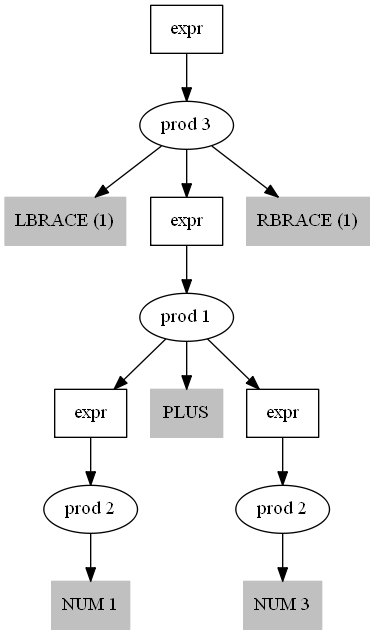
\includegraphics{Ivanov/Pictures/Dynamic_DynamicRes1.png}
    }
    \qquad \qquad
    \subfloat[]{
        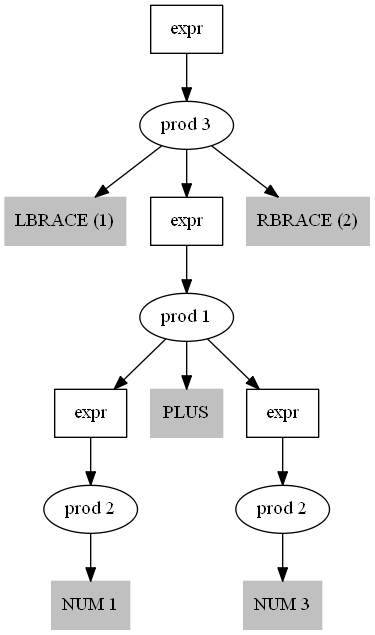
\includegraphics{Ivanov/Pictures/Dynamic_DynamicRes2.png}
    }
    \caption{Результат алгоритма для динамической подсветки.}
    \label{dynamicRes}
\end{figure}

Таким образом, если курсор стоит перед парным токеном, то нам нужно вернуть ровно n деревьев, где n~--- количество пар данного токена. 

Поскольку алгоритмы во многом пересекаются, решено было модифицировать алгоритм для статической подсветки следующим образом. 

В качестве входа алгоритм принимает два параметра:
\begin{itemize}
\item root~--- корень графа разбора;
\item токен t, пары которому нужно найти.
\end{itemize}

В ходе своей работы алгоритм сохраняет полученные деревья в множестве trees. Как и в предыдущем алгоритме, все вершины окрашены в белый цвет.

Алгоритм возвращает GetAllTreesWithToken (root, token).

GetAllTreesWithToken (root, token):
\begin{enumerate}
\item trees = $\emptyset$
\item newTree = Handle (root, token, trees)
\item пока newTree $\notin$ trees:
\item \qquad trees = trees $\cup$ \{newTree\}
\item \qquad newTree = Handle (root, token, trees)
\item вернуть trees
\end{enumerate}		
		
Handle (v, token, trees):
\begin{enumerate}
\item Если вершина v --- вершина-символ, то 
    \begin{itemize}
        \item если OutEdges (v) == 1, то Handle (Succ (v), token, trees).
        \item если OutEdges (v) > 1, то если среди u $\in$ Succ(v) $\exists$ s такой, что token $\in$~Tokens (s), то Handle (s, token, trees). 
        \item Иначе идти по такому r $\in$ Succ(v), который содержит наибольшее количество новых токенов (на фоне множества trees). 
	\end{itemize}
	Перейти к шагу 3.
\item Если текущая вершина --- вершина-продукция, то для каждой вершины u из Succ(v) сделать следующее:  Handle (u, token, trees). Перейти к шагу 3.
\item Покрасить v в чёрный цвет. Если v == root, то перейти к шагу 4.
\item Алгоритм завершает работу. Вернуть дерево, состоящее из ``чёрных'' вершин. 
\end{enumerate}

Иллюстрация работы алгоритма продемонстрирован на рисунке~\ref{ex}.

\begin{figure}[t]
    \centering
    % \begin{subfigure}[h]{0.25\textwidth}
    %     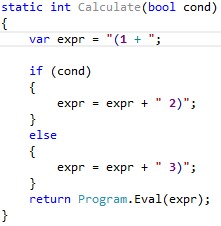
\includegraphics{Ivanov/Pictures/BracketExampleWithoutCaret.PNG}
    %     \caption*{Без курсора.}
    % \end{subfigure}
    % \\
    \subfloat[Курсор перед открывающей скобкой]{
        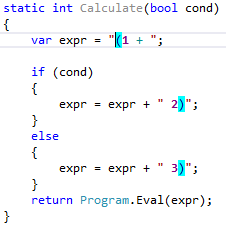
\includegraphics{Ivanov/Pictures/BracketExample.png}
    }
    \qquad \qquad \qquad
    \subfloat[Курсор после закрывающей скобки]{
        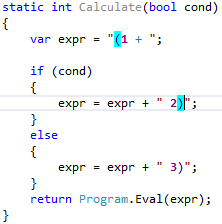
\includegraphics{Ivanov/Pictures/BracketExampleWithRight.png}
    }
    \caption{Иллюстрация работы алгоритма с подсветкой скобок.}
    \label{ex}
\end{figure}

\section{Особенности реализации}
\subsection{Изменения в генераторе}

В генератор добавлены два ключа: -highlighting и -namespace. Значение первого ключа говорит, нужна или нет подсветка. Второй ключ служит больше для технических целей соответствует имени namespace’а в сгенерированных файлах на языке C\#.

Если ключ highlighting отсутствует или же имеет значение false, то генератор отработает в обычном режиме и вернёт только парсер этой грамматики. 

Если ключ highlighting имеет значение true, то помимо стандартных преобразований надо грамматикой (таких как раскрытие правил EBNF) будут произведены дополнительные. Они направлены на то, чтобы для каждого правила сгенерировать семантику для подсветки. Если же во входной грамматике была определена пользовательская семантика, то она ``затирается'', а на ее место ставится семантика подсветки. 

\begin{figure}[t]
\centering
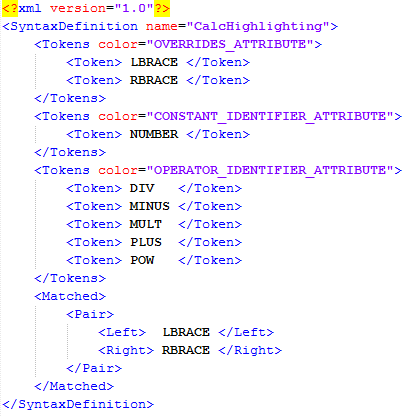
\includegraphics{Ivanov/Pictures/xmlExample.PNG}
\caption{Пример xml файла.}
\label{xml}
\end{figure}

Поскольку в общем случае неизвестно, какие терминалы будут во входной грамматике и соответственно в какой цвет каждый из них подсвечивать, то автоматизировать привязку к каждому токену определенного цвета невозможно. Поэтому решено на этом этапе также возвращать xml-файл (см. рис.~\ref{xml}). Он содержит в себе сопоставление ``токен -> цвет''. Также в нём поддерживается задание парных символов, что позволяет осуществлять динамическую подсветку (например, для открывающих и закрывающих скобок). 

В генераторе используются цвета, принятые в ReSharper SDK. Для удобства пользователя названия всех доступных цветов указываются в комментариях сгенерированного xml файла. 
\subsection{Архитектура решения}

Общая архитектура решения изображена на~\ref{architecture}. Серым цветом отмечены модули, которые были созданы либо изменены в ходе данной работы.

\begin{figure}[t]
\centering
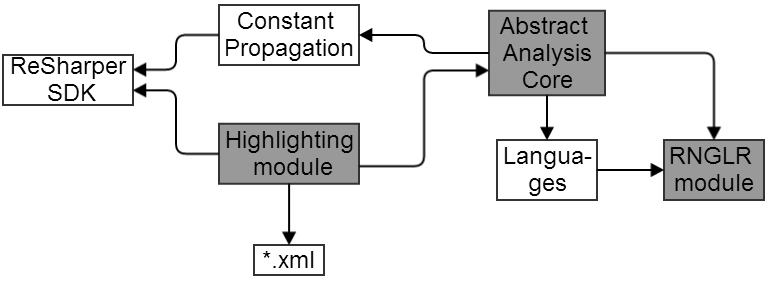
\includegraphics[width=\linewidth]{Ivanov/Pictures/architecture.png}
\caption{Архитектура решения.}
\label{architecture}
\end{figure}

Рассмотрим эти модули поподробнее. 

Модуль RNGLR содержит в себе функции для работы с графом разбора. В частности он включает реализацию описанных в предыдущей главе алгоритмов извлечения деревьев из SPPF. 

Модуль Languages содержит в себе информацию, специфичную для каждого языка. Например, у каждого языка свой алфавит, свой синтаксический анализатор, своя функция вычисления семантики. Именно такую информацию Languages и хранит. 

Работа модуля AbstractAnalysisCore проходит в два этапа. 

\begin{figure}[t]
\centering
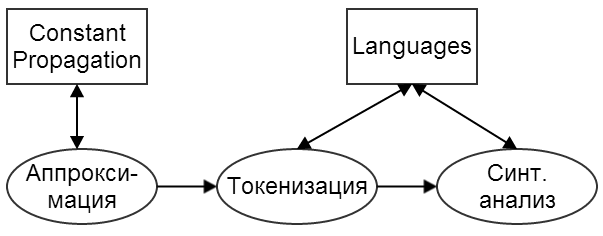
\includegraphics[width=\linewidth]{Ivanov/Pictures/Core.png}
\caption{Анализ файла модулем AbstractAnalysisCore.}
\label{core}
\end{figure}

На первом этапе происходит анализ файла (рисунок~\ref{core}). Сперва проходит аппроксимация множества значений строковых выражений, для чего используется другой модуль --- ConstantPropagation, целью которого является протягивание констант. Результатом аппроксимации является граф, на рёбрах которого находятся фрагменты строк исходного файла. Также с графом ассоциируется язык, которому соответствуют строки. Далее происходит токенизация полученного графа, в результате которой получается граф, на рёбрах которого находятся токены, а не строки. После токенизации происходит синтаксический анализ. Результат синтаксического анализа --- граф разбора --- сохраняется. 

\begin{figure}[t]
\centering
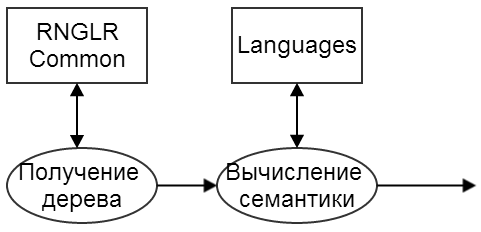
\includegraphics[width=\linewidth]{Ivanov/Pictures/Core_GetTree.png}
\caption{Получение дерева в AbstractAnalysisCore.}
\label{core_tree}
\end{figure}

На втором этапе работы модуля AbstractAnalysisCore происходит генерация деревьев. Этот этап проиллюстрирован на рисунке~\ref{core_tree}. Для получения дерева используется модуль RNGLRCommon, который был описан ранее. После того, как дерево получено, происходит вычисление его семантики, и возвращается полученный результат. 

Наконец, модуль Highlighting отвечает за подсветку и интеграцию с ReSharper SDK. Он состоит из трёх подмодулей. Один из них отвечает за статическую подсветку, второй --- за динамическую подсветку, а третий (Helper) служит для взаимодействия между ними. 

\begin{figure}[t]
\centering
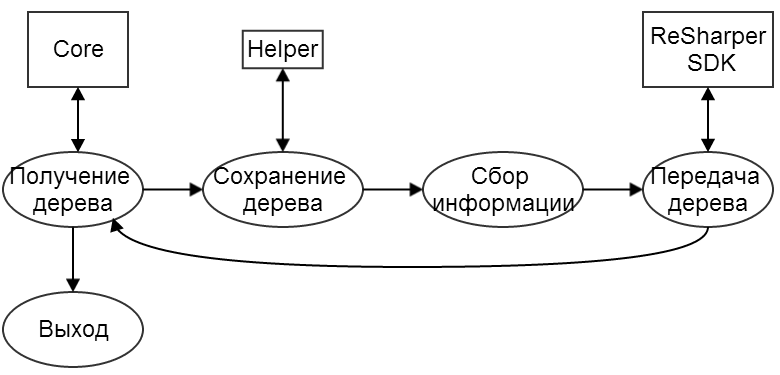
\includegraphics[width=\linewidth]{Ivanov/Pictures/staticHighlighting.png}
\caption{Схема работы модуля статической подсветки.}
\label{staticHighlighting}
\end{figure}

Схема работы подмодуля, занимающегося статической подсветкой, изображена на рисунке~\ref{staticHighlighting}. Этот подмодуль начинает работу при каждом изменении файла с исходным кодом. Такое поведение достигается за счёт установления соответствующего атрибута в одном из классов этого подмодуля. Контекст при этом не учитывается. Модуль создаёт инстанцирует класс AbstractAnalysisCore, который проводит синтаксический анализ кода на встроенном языке. После этого возвращается дерево разбора, полученное согласно алгоритму, описанному в разделе 3.2.1. Полученное дерево сохраняется в Helper’е. Далее происходит обход этого дерева, в ходе которого происходит сбор информации о том, какой токен на какой позиции в файле находится. Также каждому токену назначается цвет, в который этот цвет красить (здесь всплывает xml файл, который описан в предыдущем разделе). После этого полученная информация передаётся ReSharper SDK, который осуществляет непосредственную подсветку. И начинается запрос нового дерева. Процесс продолжается до тех пор, пока полученное дерево не является пустым.

\begin{figure}[t]
\centering
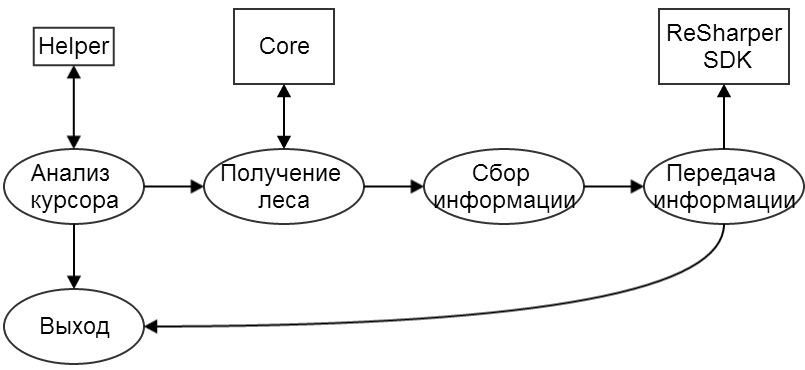
\includegraphics[width=\linewidth]{Ivanov/Pictures/dynamicHighlighting.png}
\caption{Схема работы модуля динамической подсветки.}
\label{dynamicHighlighting}
\end{figure}

Схема работы подмодуля, занимающегося динамической подсветкой, выглядит несколько иначе (рисунок~\ref{dynamicHighlighting}). В отличие от предыдущего модуля он реагирует на каждое изменение положения каретки курсора в файле с исходным кодом. При запуске этого подмодуля сперва происходит анализ положения курсора. Если каретка стоит внутри строкового выражения и перед (после) открывающего (закрывающего) парного символа, то определяется текущий встроенный язык. Это определение происходит за счёт поиска по деревьям разбора, полученным при статической подсветке. Сначала определяется дерево, которое содержит нужный диапазон, а потом по этому дереву определяется, какой именно это встроенный язык. На основе полученной информации у объекта класса AbstractAnalysisCore вызывается функция, которая возвращает все деревья, которые содержат нужный токен. Алгоритм, который используется при этом, описан в разделе 3.2.2. Далее по этим деревьям, так же, как и в работе подмодуля статической подсветки, происходит сбор информации и её передача ReSharper SDK, который подсвечивает парные токены. 


% У заключения нет номера главы
\section*{Заключение}

В рамках данной работы были достигнуты следующие результаты:
\begin{itemize}
\item изучены инструмент YaccConstructor и платформа ReSharper SDK.
\item создан алгоритм подсветки произвольных встроенных языков, описанных грамматикой;
\item реализован и апробирован полученный алгоритм;
\item результаты группы, в которую входит автор, приняты на семинар ``Наукоёмкое программное обеспечение''.
\end{itemize}

В дальнейшем планируется реализация так называемой семантической подсветки --- подсветки, которая основывается на некоторых дополнительных свойствах программы. 

На рисунке~\ref{dead_code} продемонстрирован один из примеров такой подсветки --- подсветка ``мёртвого кода''. Как можно заметить, те фрагменты кода, которые не имеют смысла, окрашены серым цветом, вне зависимости от типа языковых конструкций.

\begin{figure}[t]
\centering
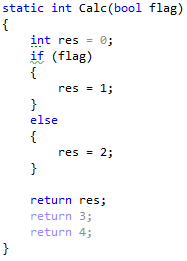
\includegraphics{Ivanov/Pictures/dead_code.PNG}
\caption{Семантическая подсветка в ReSharper.}
\label{dead_code}
\end{figure}

Другим направлением является реализация других возможностей современных IDE по отношению ко встроенным языкам. Например, средства навигации по коду (find usage, goto definition), автодополнение, анализ корректности типов. 

\begin{thebibliography}{99}
\bibitem{RNGLR}
Elizabeth Scott, AdrianJohnstone.
Right Nulled GLR Parsers //
ACM Transactions on Programming Languages and Systems (TOPLAS), Vol.~28, 2006.

\bibitem{FSharp}
Don Syme, Adam Granicz, Antonio Cisternino.
Expert F\# 3.0, 2012.

\bibitem{JSA}
Aske Simon Christensen, Anders Moller, Michael I.Schwartzbach".
Precise Analysis of String Expressions //
Proceedings of 10th International Symposium on Static Analysis, 2003.

\bibitem{PSA}
Y. Minamide. Static Approximation of Dynamically Generated Web Pages //
Proceedings of the 14th international conference on World Wide Web, 2005.

\bibitem{ARNGLR}
Semyon Grigoriev, Iakov Kirilenko. GLR-based abstract parsing //
Proceedings of the 9th Central \& Eastern European Software Engineering Conference in Russia, 2013.

\bibitem{Kim}
Kinm Hyunha, Doh Kyung-Goo, Schmidt David.
Static Validation of Dynamically Generated HTML Documents Based on Abstract Parsing and Semantic Processing //
Proceedings of 20th International Symposium on Static Analysis, 2013.

\bibitem{YC_paper}
Я.А.Кириленко, С.В.Григорьев, Д.А.Авдюхин.
Разработка синтаксических анализаторов в проектах по автоматизированному реинжинирингу информационных систем //
Научно-технические ведомости Санкт-Петербургского государственного политехнического университета. Информатика. Телекоммуникации. Управление, 2013.
\end{thebibliography}
